\chapter{Methodology}%
Construction of associative memory using \Snn\cite{base} in this method consist of four phases
\begin{enumerate}
    \item Initialization :Initialization of \Snn and the input spiking signals
    \item Structure formation :
    \item Parameter training :
    \item Pruning :
\end{enumerate}
\section{Initialization}
\subsection{Initialization input spiking signals}
\begin{figure}[h!]
    \centering
    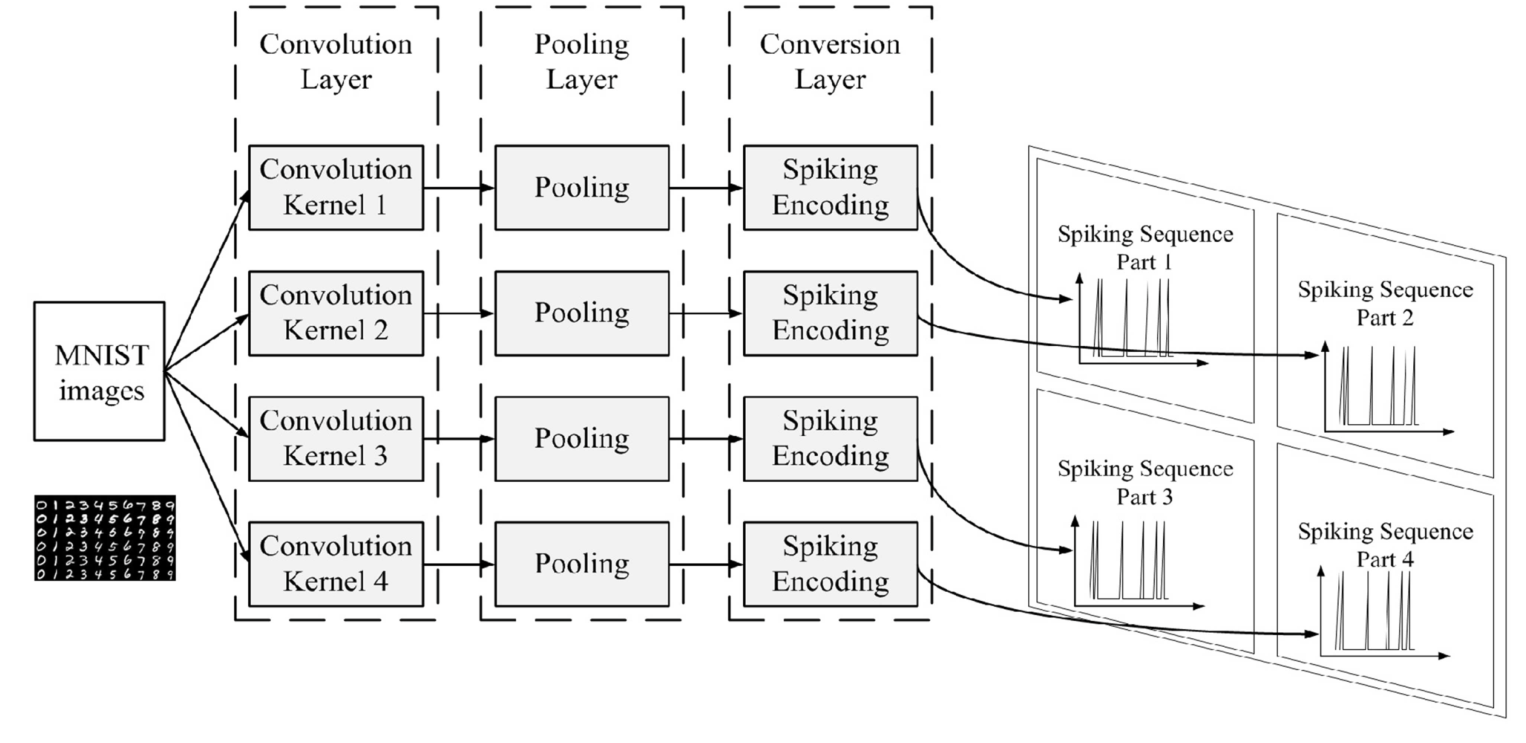
\includegraphics[width=0.7\linewidth]{preprocessing}
    \caption{Data preprocessing}
    \label{preprocessing}
\end{figure}
\begin{figure}[h!]
    \centering
    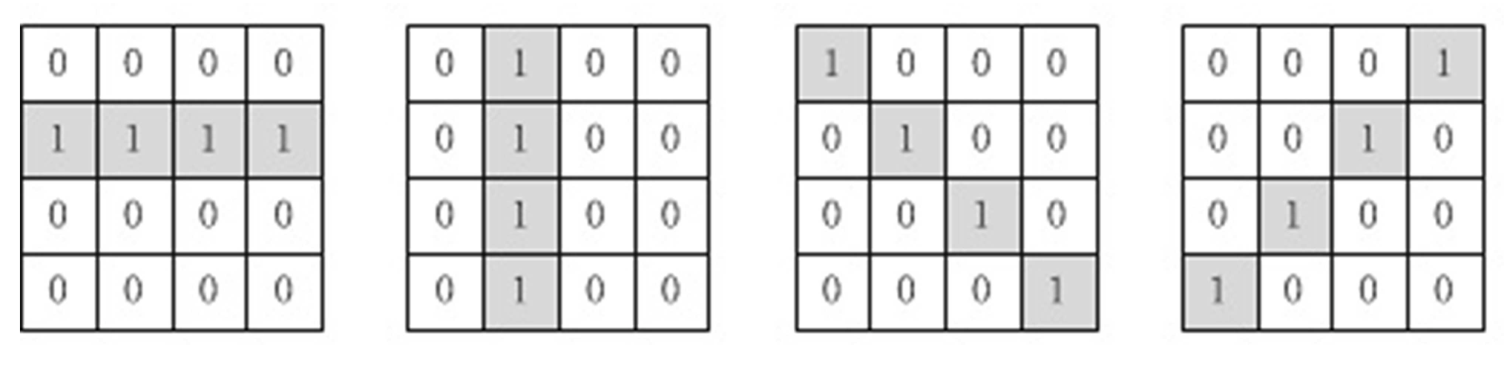
\includegraphics[width=0.7\linewidth]{kernels}
    \caption{Kernels used}
    \label{kernel}
\end{figure}
\subsection{Initialization of \Snn}
\begin{figure}[h!]
    \centering
    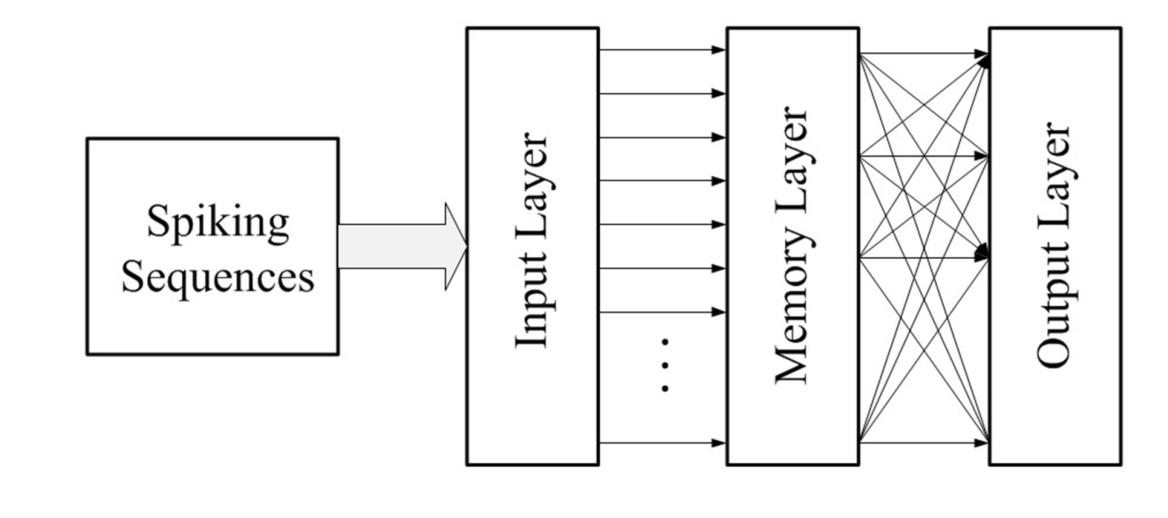
\includegraphics[width=0.7\linewidth]{structure}
    \caption{Structure of network}
    \label{structure}
\end{figure}
\begin{figure}[h!]
    \centering
    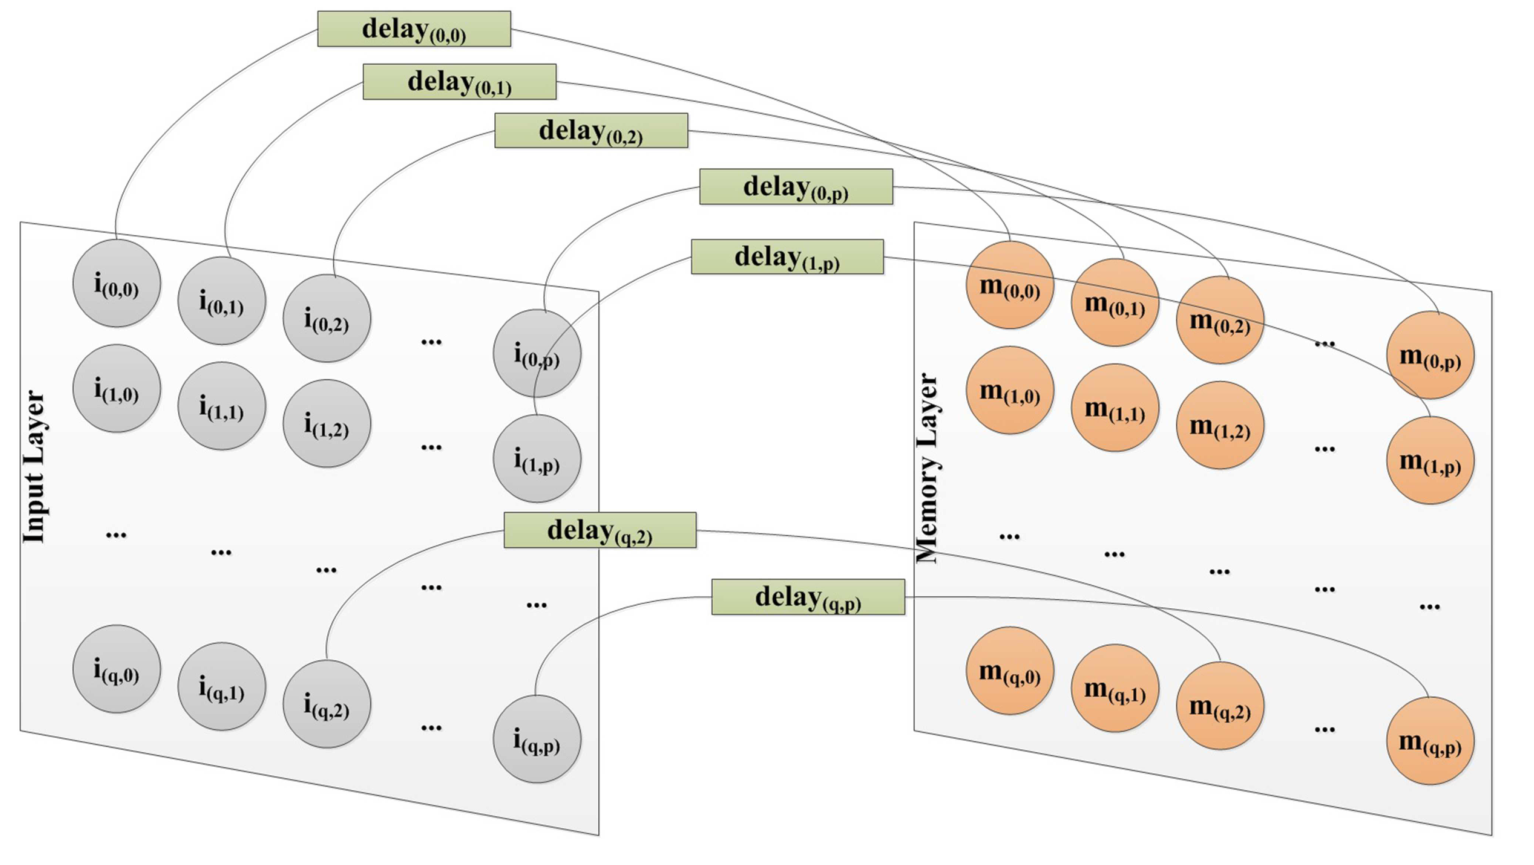
\includegraphics[width=0.7\linewidth]{delay}
    \caption{Delay for neuron}
    \label{delay}
\end{figure}
\section{Structure formation}
\section{Parameter training}
\begin{figure}[h!]
    \centering
    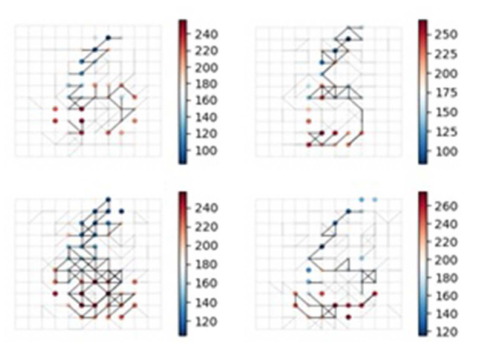
\includegraphics[width=0.7\linewidth]{recall}
    \caption{Recall response for number 6}
    \label{recall}
\end{figure}
\section{Pruning}
% This section describes the research methods used in the seminar, including the
% participants, data collection techniques, and data analysis methods.